\documentclass[bsc,singlespacing,parskip,deptreport,twoside,frontabs]{infthesis}


\usepackage{graphicx}
\begin{document}



\title{Automatic Harmonic Analysis of Jazz Solos - Report}

\author{Finlay McAfee - s1220880}

\course{Master of Informatics}
\project{{\bf MInf Project (Part 1)}}

\date{\today
}

\abstract{
Hey look an abstract.
}

\maketitle

\tableofcontents

\pagenumbering{arabic}


\chapter{Introduction and Theoretical Motivation}

The aim of this project is to build a system that will analyse a melody and determine the underlying chord sequence. The purpose of this report is to give a summary of the current progress and detail the further work that shall be done, in both this year and the expanded project next year.

The proposed system to tackle this task is based on the assumption that harmonic analysis of musical input is analogous to automatic speech recognition in the field of natural language processing. This allows the task to be divided into two distinct modules, a transition (language) model and an emission (acoustic) model. The transition model is the probability of transitioning from one chord to another. The emission model is the probability of the current chord generating the observed notes. This kind of structure allows for a probabilistic generative model, where given a chord sequence we can model the generation of the more complex note sequence.

$$
P(o_t) = P(o_t | s_t)P(s_t | s_{1:t}) 
$$

The task of the first year of this project is to design a baseline Hidden Markov Model system, where the transition model is the first order markov assumption:

$$
P(s_t | s_{1:t}) = P(s_t | s_{t-1}) 
$$

This allows the focus to be on designing an emission model that best captures the relationship between the observations and the underlying chord. This process can be split into two tasks, feature extraction and segment classification. The approach taken to both will be detailed as well as planned future improvements. 


\chapter{Current System Description}

This section outlines the current state of the proposed system. The structure of each component will be summarised, along with it's function in the complete system. For most components there are currently multiple possible models, the following chapter will then present and analyse experiments done over these variations.

\section{Emission Model}

\subsection{Feature Extraction}
This interim report presents the current state of the proposed system. This system is an automatic harmonic analysis program, taking inspiration from those used in speech processing.
\subsubsection{The Data}

The training of any classification system requires supervised data and in the field of music this can be a challenge to source due to copyright issues. Luckily for this project there is a fantastic, openly available database of annotated jazz solo transcriptions made available by The Jazzomat Research Project called the Weimar Jazz Database (WJazzD) \cite{wjazz}. The data has been made available since February 20th 2015 and was constructed using an open source audio recording analysis software called Sonic Visualiser \cite{sv}. The database contains 299 MIDI transcriptions of jazz solos by famous musicians along with the annotated meta data.

\subsubsection{Preprocessing}

The Emission Model captures the observed data with feature vectors, so the MIDI files must first be processed into these desired features. Also a useful representation must be determined for the annotated chords that are to be used as classification categories.

In western tonal music, songs are generally divided into keys. These tend to centred on of twelve possible notes, called the tonic, and are then further modified by being either major, minor or (more rarely) one of seven possible 'modes'. Key information is available for the data used in both training and testing, so to normalise for this a relative representation of pitch was chosen. Specifically each instance of a note or chord is expressed as a Tonal Pitch Class (TPC), a value between 0 and 11, which represents the distance in semitones between the note and the tonic of the piece (i.e. the key). This can be thought of as transposing all the solos to the same key. It should be noted that in doing this both a system of equal temperament is assumed, and absolute pitch data is abstracted away, hence if one note is an octave above another, they are considered the same to be the same TPC. It is possible to account for the variations in mode \cite{mysong} but that is not done at this time.

Information regarding pitch is not the only data that is useful in this task, metrical data is also used. For this information we adopt the following terminology, introduced by \cite{mel}: the songs are divided into distinct \emph{bars}; each bar in one song contains the same number of \emph{beats}, generally between two and four; each beat can be divided into any number of \emph{divisions}; each individual division is referred to as a \emph{tatum}. As additional features for each note of the melody, the \emph{beat} the note lands on, the number of \emph{divisions} on that beat, the duration of that note in tatums (the \emph{durtatum}) and the current \emph{tatum}, are all used.

On top of this, specific metrical qualities in a note are explicitly modelled. Whether or not the note is \emph{syncopated} is represented with a binary feature. The \emph{metrical weight} is represented with a ternary feature, zero for a sub-beat event, one for a weak beat event (i.e. on the 'off beat') and two for a strong beat event (i.e. on the 'on beat'). Lastly an alternative metrical system was also tested, introduced by \cite{mcm48}, which in based on a circular system with 48 divisions.

With the incorporation of sequential information in mind, models were also used where the feature vectors contained the values of the previous and next notes in the sequence as components.

The WJazzD is designed to work with music processing software created by the Jazzomat Research Project called MeloSpySuite \cite{mel}. The {\tt melfeature} tool was used to do the above preprocessing.

\subsection{Segment Classification}

The next step is to segment the data into sections to assign chords to. At the current time, to focus on choosing the best possible emission model, both the training and the test datasets have been segmented into sections of varying sizes at points where it is known there are chord transitions. This will not be the method in the final model and possible options for doing this are discussed in Chapter 4.

Another choice that must be made is how fine grained the classification is going to be in terms of the number of chord categories, K. Ideally a model that took into account all possible variations on chords would be preferable, but for the sake of model comparison K is chosen to be 24, capturing major and minor variations. The following encoding is used:

$$
En(note) = 2 * tpc(note) + 1 + type(note)
$$

Where type is 0 if major and 1 if minor. This encoding allows pseudo start and end states of 0 and $N+1$ to be used.

The initial method attempted for an emission model was a Na\"ive Bayes approach based on \cite{mysong}. This involved creating a smoothed frequency count matrix of the number of times a note was observed given a certain chord. In this model the only data that was made use of was the TPCs, where each segment is represented by a frequency distribution over the notes that occur in that section.  3 contains evaluations of each method. This is the most basic model and performed the poorest.

The next method attempted was to divide the problem into two: first determine which notes in the segment are most probable to be chord tones, second use these chord tones to determine the current chord. This was modelled as two classification tasks, where the first is a binary classification over all notes and the second is a K-class classification over all segments. Currently Support Vector Machines and Decision Trees have been implemented to perform these tasks.

\section{Transition Model}

The transition model of the system is based on a First order Markov Assumption, where in the generational model, the transition probability into the state that generates the current observations is only dependent on the previous state. In this case the states are the underlying chords. It is clear from the extended structure of a piece of music that this is an extreme generalisation and work has been done into investigating the improvements that can be made from incorporating this kind of musical structure into harmonic analysis \cite{struct}. Chapter 4 describes the work that shall be done in the second year of this project to incorporate a more complex transition model.

The training of a HMM transition model can be difficult with unsupervised data and involve Estimation Maximisation algorithms. In this case however, the transition model is simply a bigram model of chords in the training set and can be trained with a smoothed frequency count of the occurrences of each bigram.

\section{Chord Sequence Generation}

To assign a sequence of chords to each song a method of combining the transition and emission models is required. Specifically the most probably sequence of chords must be determined given the data and the chosen models. To compute this the Viterbi Algorithm was implemented, based on the description in \cite{jur}.

For testing purposes chord sequences were also produced locally, based only on the emission model. For each segment the chord with the highest emission probability was chosen.

\chapter{Evaluation and Analysis}

The results presented here are from predicting chords without a transition model. The models trained on the two-part chord tone system were a Support Vector Machine (SVM) with an RBF kernel, an SVM with a linear kernel (Lin SVM) and a Decision Tree (DT). A Naive Bayes (NB) model was also used predicting chords straight from the data.

\section{Predicting Chord Tones from Data}

The effect of feature selection were tested over there ability to predict chord tones. The ground truth was automatically computed from the annotated chords. The results are presented in Figure 3.1. 

\begin{figure}
  \caption{\textbf{Accuracy across variations on input features:} \emph{Local} refers to the use of only data from the current note. \emph{Seq} refers to use of additional data from the previous and following note. \emph{B} refers to beat information, \emph{Div} to number of divisions, \emph{D} to 'duratum' and \emph{TPC} to the tonal pitch class.}
  \centering
    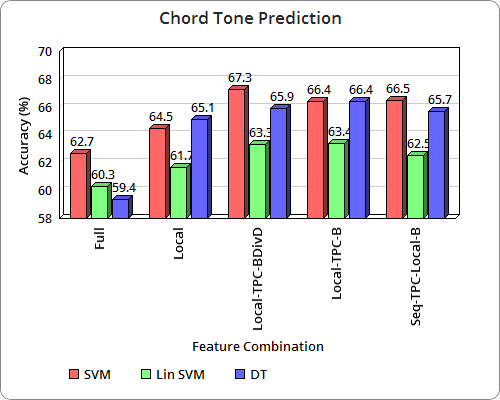
\includegraphics[scale=0.5]{ct1}
\end{figure}

From these results it is clear both that an SVM model achieves the highest accuracy and that Local-TPC-BDivD (see Figure 3.1) was the best combination of features.

\section{Predicting Chords from Chord Tones}

The input to the learner that takes chord tones to chords is a 12-dim vector for each segment, with each component representing a TPC. Two methods of input were tested, one where each component is a binary indicator of whether the corresponding note is a chord tone in this segment, the other where it is a frequency count of the number of times that note appears as a chord tone in this segment, putting more weight on that note. The results are shown in Figure 3.2.

\begin{figure}
  \caption{\textbf{Accuracy across variations on chord tone representation:} \emph{Bin} refers to the binary representation and \emph{Freq} to the frequency.}
  \centering
    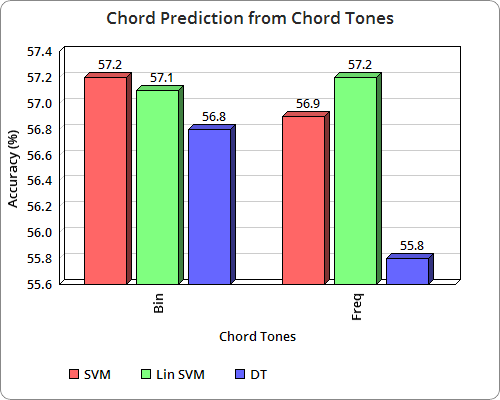
\includegraphics[scale=0.5]{ch}
\end{figure}

The results show that the binary representation is preferable, again with the SVM providing the highest accuracy.

\section{Overall Performance of Local Emission Model}

Finally tests were performed combining the systems and compared to a one stage Na\"ive Bayes system and a baseline uniform probability over all classes model. Figure 3.3 shows the accuracies and Figure 3.4 contrasts the performance time of each system.

\begin{figure}
  \caption{\textbf{Full Emission Model}}
  \centering
    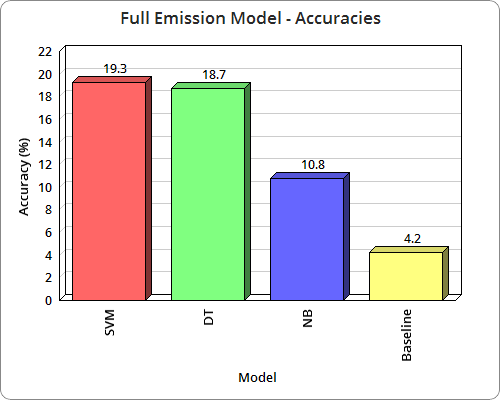
\includegraphics[scale=0.5]{em}
\end{figure}

\begin{figure}
  \caption{\textbf{Training and Testing Times}}
  \centering
    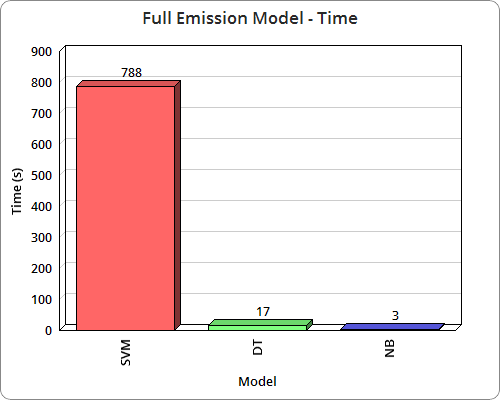
\includegraphics[scale=0.5]{time}
\end{figure}

It is noted that these accuracies are not competitive, but their enhanced performance over a baseline model of uniform chance shows that they represent the emission relationship to some degree.

\chapter{Conclusion and Further Work}

\section{Remaing Work of Part 1}

The nest step is to perform the experiments from the previous chapter while incorporating the transition model into the prediction system.

Currently a method of incorporating local sequential data into the emission model is being investigated. One possibility is to use a Recurrent Neural Network (RNN) for segment classification, where the input is the sequence of notes in that segment.

Another task is to segment the data automatically. One method that will be attempted is to treat each note as an individual segment and assign a chord to each note, with consecutive assignments of the same chord being treated as one chord in the output sequence. This restricts what can be achieved with the emission model and puts more weight on the transition probabilities. Another method is to uniformly segment the data into sections of equal size, e.g. a bar.

More machine learning methods for segment classification will also be implemented, including CRFs, Neural Networks and Gaussian Mixture Models.

Finally further experiments shall be carried out over different variations of the system to test the various parameters and find the most successful model.

\section{Part 2}

The primary purpose of the second year of this project is to investigate the effects extended structural analysis with more complex transition models.

One proposed method is to adapt a jazz parser presented by \cite{ccg}
 that currently uses Combinatory Categorical Grammars (CCGs) to analyse jazz chord sequences. As it is a statistical model, it could be adapted to give probabilities of individual chord sequences. This could be combined with an emission model of notes to chords to create a system that could search for the overall most probable harmonic analysis.

Other language models that take into account extended sequential structure and context are those involving Recurrent Neural Networks (RNNs) \cite{rnn}. An RNN based approach will also be implemented, in comparison with the grammar model.

\section{Final Remarks}

In this report the current state of an NLP informed harmonic analysis system has been presented, with details of experiments carried out and further work planned. The final report for this year's work on the project will be presented on Thursday 31st of March, followed by a presentation in the week beginning April 25th.


% use the following and \cite{} as above if you use BibTeX
% otherwise generate bibtem entries
\begin{thebibliography}{9}
\bibitem{wjazz}
 Abeßer, J., Frieler. K., Pfleiderer, M., \& Zaddach, W.-G. (2013). Introducing the Jazzomat project - Jazz solo analysis using Music Information Retrieval methods. \emph{Proceedings of the 10th International Symposium on Computer Music Multidisciplinary Research (CMMR) Sound, Music and Motion, Marseille, Frankreich.}

\bibitem{sv}
Cannam, C., Landone, C., \& Sandler, M. (2010, October). Sonic visualiser: An open source application for viewing, analysing, and annotating music audio files. \emph{Proceedings of the international conference on Multimedia (pp. 1467-1468). ACM.}

\bibitem{mysong}
Simon, I., Morris, D., \& Basu, S. (2008, April). MySong: automatic accompaniment generation for vocal melodies. \emph{Proceedings of the SIGCHI Conference on Human Factors in Computing Systems (pp. 725-734). ACM.}

\bibitem{mel}
Frieler, K., Abeßer, J., Zaddach, W.-G., \& Pfleiderer, M. (2013). Introducing the Jazzomat Project and the Melo(S)py Library. In: Kranenburg, P. van, Anagnostopoulou, C., \& Volk, A. (Ed.) \emph{Proceedings of the Third International Workshop on Folk Music Analysis, Meertens Institute and Utrecht University Department of Information and Computing Sciences, pp. 76–78.}

\bibitem{mcm48}
Frieler, K. (2007, September). Visualizing Music on the Metrical Circle. \emph{ISMIR (pp. 291-292).}

\bibitem{struct}
Mauch, M., Noland, K., \& Dixon, S. (2009). Using Musical Structure to Enhance Automatic Chord Transcription. \emph{ISMIR (pp. 231-236).}

\bibitem{jur}
Martin, J. H., \& Jurafsky, D. (2000). Speech and language processing. International Edition.

\bibitem{ccg}
Granroth-Wilding, M., \& Steedman, M. (2012). Statistical parsing for harmonic analysis of jazz chord sequences. \emph{Ann Arbor, MI: MPublishing, University of Michigan Library.}

\bibitem{rnn}
Mikolov, T., Karafiát, M., Burget, L., Cernocký, J., \& Khudanpur, S. (2010, January). Recurrent neural network based language model. \emph{INTERSPEECH 2010, 11th Annual Conference of the International Speech Communication Association, Makuhari, Chiba, Japan, September 26-30, 2010 (pp. 1045-1048).
Chicago}


\end{thebibliography}

\end{document}
